\documentclass[tikz,border=3.14pt]{standalone}
\usetikzlibrary{3d,decorations.text,shapes.arrows,positioning,fit,backgrounds,arrows}
% from https://tex.stackexchange.com/a/52856/121799
\tikzset{circle dotted/.style={dash pattern=on .05mm off 2mm,
                                         line cap=round}}
\begin{document}

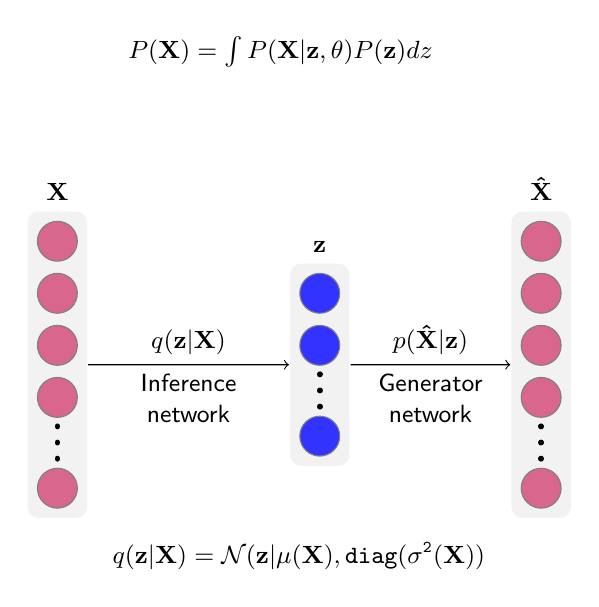
\begin{tikzpicture}[font=\sffamily\small,scale=2]

\node[circle,draw,gray,fill=purple!60] (A1) at (0,0,0) {~~~};
\node[circle,draw,gray,fill=purple!60,below=4pt of A1] (A2) {~~~};
\node[circle,draw,gray,fill=purple!60,below=4pt of A2] (A3) {~~~};
\node[circle,draw,gray,fill=purple!60,below=4pt of A3] (A4) {~~~};
\node[circle,draw,gray,fill=purple!60,below=18pt of A4] (A5) {~~~};
\draw[circle dotted, line width=2pt,shorten <=3pt] (A4) -- (A5);


\node[circle,draw,gray,fill=blue!80,right=80pt of A2] (B1) {~~~};
\node[circle,draw,gray,fill=blue!80,below=4pt of B1] (B2) {~~~};
\node[circle,draw,gray,fill=blue!80,below=18pt of B2] (B3) {~~~};
\draw[circle dotted, line width=2pt,shorten <=3pt] (B2) -- (B3);

\node[circle,draw,gray,fill=purple!60, right=160pt of A1] (C1) {~~~};
\node[circle,draw,gray,fill=purple!60, below=4pt of C1] (C2) {~~~};
\node[circle,draw,gray,fill=purple!60, below=4pt of C2] (C3) {~~~};
\node[circle,draw,gray,fill=purple!60, below=4pt of C3] (C4) {~~~};
\node[circle,draw,gray,fill=purple!60, below=18pt of C4] (C5) {~~~};
\draw[circle dotted, line width=2pt,shorten <=3pt] (C4) -- (C5);


\begin{scope}[on background layer]
\node[label={${\bf X}$},gray,thick,rounded corners,fill=gray!10,fit=(A1) (A5)] (AA1) {};
\node[label={${\bf z}$},gray,thick,rounded corners,fill=gray!10,fit=(B1) (B3)] (BB1) {};
\node[label={${\bf \hat{X}}$},gray,thick,rounded corners,fill=gray!10,fit=(C1) (C5)] (CC1) {};
\end{scope}
%\foreach \X in {1,2,3}
%{\draw[-latex] (A\X) -- (B2);}
\draw[->] (AA1) -- (BB1) node[midway,above] {$q({\bf z}|{\bf X})$} node[align=center, midway,below] {Inference \\ network};
\draw[->] (BB1) -- (CC1) node[midway,above] {$p({\bf \hat{X}}|{\bf z})$} node[align=center,midway,below] {Generator \\ network};

\node[text width=5cm] at (1.7,1.2)
    {$P({\bf X}) = \int P({\bf X}|{\bf z},\theta)P({\bf z})dz$};
\node[text width=5cm] at (1.6,-2) 
    {$q({\bf z}|{\bf X}) = \cal{N}({\bf z}|{\bf \mu}({\bf X}), \tt{diag}({\bf \sigma}^2({\bf X}))$};

\end{tikzpicture}



\end{document}
